% !TEX root = ../cnf-json.tex
The first component of \systemnametwo, the schema pane, shows the relational schema of the extracted view.
Initially, this schema consists of one attribute for every path in the \json collection being summarized.
Attributes may be deleted or restored, and sets of attributes may be unified.

The core challenge behind implementing this pane is that, depending on data set, the schema could consist of hundreds or thousands of attributes.
This can be overwhelming for users who just wants to find account profiles appearing in a Twitter stream.
To mitigate this problem, \systemnametwo presents the schema in a summarized form.

Specifically, attributes are grouped based on both correlations and anti-correlations between them.
Groups of \emph{correlated} attributes, or those that frequently co-occur in \json records are likely to be part of a common structure.
Similarly, groups of \emph{anti-correlated} attributes, or those that rarely co-occur in \json records are likely to represent alternatives (e.g., a Street Address vs GPS coordinates).  
We use correlations and anti-correlations between attributes to compact the schema for representation.
Before describing the summary itself, we first formalize the problem.

%%%%%%%%%%%%%%%%%%%%%%%%%%%%%%%%%%%%%%%%%%%%%%%%%%%%%%%%%%%%%%%%%%%%

\subsection{Data Model}
A \json object is an order-independent mapping from keys to values.
A key is a unique identifier of a \json object, typically a string.
A value may be atomic or complex. 
Atomic values in \json may be integers, reals, strings, or booleans.
A complex value is either a nested object, or an \textit{array}, an indexed list of values.  
For simplicity, we model arrays as objects by treating array indexes as keys.
A \json record may be any value type, but for simplicity of exposition we will assume that all records are objects.  
\begin{example}
\label{example:jsonobject}
A fragment of Twitter Tweet encoded as \json
\begin{lstlisting}[language=json]
"tweet": {
  "text": "#SIGMOD2018 in Houston this year",
  "user": { 
    "name" : "Alice Smith",  "id" : 12345, 
    "friends_count": 1023,  …
  },
  "retweeted_status": {
    "tweet": {
      "user": { … }, "entities": { … }, 
      "place": { … }, "extended_entities": { … }
    }, …
  },
  "place": { … }, "extended_entities": { … },  
  "entities": { "hashtags": [ "SIGMOD2018" ], … },
  …
}
\end{lstlisting}
\end{example}

\noindent 
\json objects are typically viewed as trees with atomic values at the leaves, complex values as inner nodes, and edges labeled with the keys of each child.
Our goal is to identify commonalities in the structure of this tree across multiple \json records in a collection.  
To capture the structure, we define the \textit{schema} $S$ of a \json record as the record with all leaf values replaced by a constant $\bot$.
A \emph{path} $P$ is a sequence of keys $P = (k_0, \ldots, k_N)$.
For convenience, we will write paths using dots to separate keys (e.g., \inlinejson{tweet.text}).
We say that a path appears in a schema (denoted $P \in S$) if it is possible to start at the root of $S$ and traverse edges in order. 
If the value reached by this traversal is $\bot$, we say that $P$ is a terminal path of $S$ (denoted $P \bot S$).

\subsection{Paths as Attributes}
Ultimately, our goal is to create a flat, relational representation suitable for use with an entire collection of \json records.
The first step to reaching this goal is to flatten individual \json schemas into collections of attributes.
We begin with a naive translation where each attribute corresponds to one terminal path in the schema.
We write $S^\bot$ to denote the path set, or relational schema of \json schema $S$, defined as:
$
S^\bot = \comprehension{P}{P \bot S}
$
Since keys are unique, commutative and associative, this representation is interchangeable\footnote{modulo empty objects or arrays} with the tree representation.
Hence, when clear from context we will abuse syntax, using $S$ to denote both a schema and its path set.
% Hence, without loss of generality, from this point on we refer to terminal path sets as just schemas.
\begin{example}
The path set of the \json object from Example~\ref{example:jsonobject} includes the paths:
\begin{enumerate*}
  \item \inlinejson{tweet.text} \;
  \item \inlinejson{tweet.user.friends\_count}
  \item \inlinejson{tweet.user.id}\;
  \item \inlinejson{tweet.entities.hashtags.[0]}
\end{enumerate*}
Each terminal appears in the set.  Note in particular that single element of the array at \inlinejson{tweet.entities.hashtags} is assigned the key \inlinejson{[0]}.
\end{example}
Path sets make it possible to consider containment relationships between schemas.  
We say that $S_1$ is contained in $S_2$ iff $S_1^\bot \subseteq S_2^\bot$.

%%%%%%%%%%%%%%%%%%%%%%%%%%%%%%%%%%%%%%%%%%%%%%%%%%%%%%%%%%%%%%%%%%%%

\subsection{Schema Collections}
We now return to our main goal, summarizing the schemas of collections of \json records.  
The starting point for this process is the schemas themselves.  
Given a collection of \json records, we can extract the set of schemas $\{\;S_1, \ldots, S_N\;\}$ of records in the collection, which we call the \emph{source schemas}.
One existing technique for summarizing these records, used by Oracle's JSON Data Guides~\cite{oracledataguide,DBLP:conf/sigmod/LiuHMLC16}, is to simply present the set of all paths that appear anywhere in this collection.
We call this the \emph{joint schema} $\mathbb S$:
$$\mathbb S^\bot \;\;\; \defineeq \;\;\; \bigcup_i S_i^\bot$$
Observe that, by definition, each of the source schemas is contained in the joint schema.
The joint schema mirrors existing schemes for relational access to JSON data like  for example.  
However, the joint schema can still be very large, with hundreds, thousands, or even tens of thousands of columns\footnote{One dataset~\cite{pharmadata} achieved 2.4~thousand paths through nested collections of objects.}.
To summarize them we need an even more compact encoding for sets of schemas.  

\tinysection{A Schema Algebra}
As a basis for compacting schema sets, we define a simple algebra.
Recall that we are particularly interested in summarizing cooccurrence and anti-cooccurence relationships between attributes.
$$\mathbf{A}\;\;:=\;\;\mathbf{P}\;\;|\;\;\emptyset\;\;|\;\;\mathbf{A} \wedge \mathbf{A}\;\;|\;\;\mathbf{A} \vee \mathbf{A}$$
Expressions in the algebra construct sets of schemas from individual attributes.
There are two types of leaf expressions in the algebra:
A single terminal path $P$ represents a singleton schema ($\big\{\{P\}\big\}$), while $\emptyset$ denotes a set containing no schemas $\big\{\big\}$.
Disjunction acts as union, merging its two input sets:
$$
\{\;S_1, \ldots, S_N\;\} \vee \{\;S'_1, \ldots, S'_M\;\} 
\defineeq
\{\;S_1, \ldots, S_N, S'_1, \ldots, S'_M\;\}
$$
Disjunction models anti-correlation: The resulting schema set is effectively a collection of schema alternatives.  
For example, $P_1 \vee P_2$ indicates two alternative schemas: $\{P_1\}$ or $\{P_2\}$.
Conjunction combines schema sets by cartesian product:
{\small
$$
\{\;S_1, \ldots, S_N\;\} \wedge \{\;S'_1, \ldots, S'_M\;\} 
\defineeq 
\comprehension{ S_i \cup S'_j}{ i \in [1,N], j \in [1, M] }
$$
}
Conjunction models correlations: The resulting schema set mandates that exactly one option from the left-hand-side and one option from the right-hand-side be present.
On singleton inputs, the result is also a singleton.
For example, $P_1 \wedge P_2$ is a single schema that includes both $P_1$ and $P_2$.  
For inputs larger than one element, the conjunction requires one choice from each input.
For example, $(P_1\vee P_2)\wedge(P_3 \vee P_4)$ is the set of all schemas consisting of one of $P_1$ or $P_2$, and also one of $P_3$ or $P_4$.

Although we omit the proofs for conciseness, both $\wedge$ and $\vee$ are commutative and associative, and $\vee$ distributes over $\wedge$\footnote{To be precise, the structure $\tuple{\big\{\{\mathbf P\}\big\}, \vee, \wedge, \emptyset, \big\{\{\}\big\}}$ is a semiring.}.
For conciseness, we use the following syntactic conventions:
(1)~When clear from context, a schema $S$ denotes its own singleton set, and (2)~We write $P_1P_2$ to denote $P_1 \wedge P_2$.

This schema algebra gives us a range of ways to represent schema sets.
At one extreme, the set of source schemas arrives in what is effectively disjunctive normal form (DNF).
One schema may be expressed as a conjunction of its elements, and the full set of source schemas can be constructed by disjunction.
For example, the source schemas $\{P_1, P_2\}$ and $\{P_2, P_3\}$ may be represented in the algebra as $P_1P_2 \vee P_2P_3$.

At the other extreme, the joint schema is a superset of all of the source schemas.
It too can be thought of as a schema set, albeit one that loses information about which attributes appear in which schemas.
Hence, this joint schema set may be defined as the power set of all attributes in the joint schema.
$$2^{\mathbb S} = \bigwedge_{P \in \mathbb S} (P \vee \emptyset)$$
Observe that at a minimum, each of the source schemas must appear in this schema set ($S_i \in 2^{\mathbb S}$).
However many other schemas appear in the resulting schema set as well.

% We start from the original representation of the schema distribution.
% Continuing Example~\ref{example:Log}, each schema in the example can be interpreted as a \textit{conjunction} over its set of attributes, e.g. $\vec v_1= (x_1\land x_2\land \neg x_3)$.
% Uniformly drawn from the log, a schema $\vec v$ can either be $\vec v_1$, $\vec v_2$ or $\vec v_3$.
% Namely the log is essentially a \textit{disjunction} over its schema $L= (\vec v_1\lor \vec v_2 \lor \vec v_3)$.
% We will then show that there is an general algebraic structure (i.e, commutative semiring) that can describe all schema distributions.
% To represent absence of some attributes in a more compact way other than listing their negation, we define a distinguished element $1$ or empty attribute $\emptyset$ such that $\vec v \land \emptyset=\vec v$. 
% In most cases, the distinguished element $1$ is omitted. 
% For example, $\vec v_1=(x_1\land x_2)$ which implies that all other attributes \textit{except for} $x_1,x_2$ exist in the schema. 
% In addition, to merge two logs where one is empty, we define a distinguished element $0$ or empty attribute set $\{\}$ such that  $\vec v \lor \{\}= \vec v$.
% The logs of \json schema can thus be interpreted as a polynomial with respect to the semiring $\tuple{A,\land,\lor,\{\},\emptyset}$ over the space of attributes $A$.

% \tinysection{Factorization}
% The original polynomial representation can be too verbose. 
% Notice that attribute $x_1=1$ is shared by all schemas in Example~\ref{example:Log}.
% We can thus \textit{factorize} the polynomial into
% $$
% L =x_1\land (x_2\lor x_2\lor x_3)
% $$
% Note $x_2$ is duplicated in disjunction.
% We can further reduce the verbosity by introducing frequencies
% $$
% L = x_1\cdot (\frac{2}{3}\cdot x_2+ \frac{1}{3}\cdot x_3)
% $$
% Note that we replace $\land,\lor$ with $\cdot,+$ for notation consistency.
% By using above representation, the schema distribution $p(V\;|\;L)$ for Example~\ref{example:Log} can be compactly interpreted as "$x_1$ always exists while $x_2, x_3$ alternatively co-exist with $x_1$ with probability $\frac{2}{3}, \frac{1}{3}$ respectively".

% \tinysection{Polynomial Modification}
% In cases where even the optimal factorization is still too verbose, we may want to edit the polynomial, delete or insert some terms.
% For example, consider the polynomial $f_0\cdot (\frac{1}{n}\cdot f_1+\ldots +\frac{1}{n}\cdot f_n)$ where $n$ is considerably large.
% It shows that each $f_i, i=1,\ldots,n$ does not co-exist with $f_0$ very often and in some cases it is tolerable to simply ignore them.
% In other words, we modify each term in the polynomial and delete features other than $f_0$.
% This leads to a lossy representation and we will discuss how to measure the degree of information loss in Section~\ref{}\todo{}.

% \tinysection{Pattern-based Summary}
% In most cases, we seek for a compact representation that preserves frequently shared \textit{patterns} as much as possible.
% More formally, we define a pattern as any set of features $\vec v'$ (i.e., partial schema) that may be contained in some schema $\vec v$ in the log.

% \tinysection{Summary Verbosity}

% \tinysection{Definition of Information Loss}


%%%%%%%%%%%%%%%%%%%%%%%%%%%%%%%%%%%%%%%%%%%%%%%%%%%%%%%%%%%%%%%%%%%%

\subsection{Summarizing Schema Collections}
These two extreme representations (the raw source schemas and the joint schema set) are bad, but for subtly different reasons.
In both cases, the representation is too verbose.
In the former case verboseness stems from redundancy, with significant overlap in variables between the source schemas.
Conversely in the latter case it stems from imprecision, as the schema set encompasses schemas that do not appear in the source schemas.
Of the two, the latter is more compact, in particular because each attribute appears no more than once.
This is a distinct representational advantage because the joint schema can be displayed simply as a list.

We would like to preserve this only-once property.
Our aim then, is to derive an algebraic expression (1) in which each attribute appears exactly once, and (2) that is as tight a fit to the original source schema set as possible.
Ultimately, this problem reduces to polynomial factorization and the discovery of read-once formulas~\cite{Dalvi:2013:DPI:2395116.2395119}, a problem that is, in general, worse than P-time~\cite{DBLP:conf/focs/Burgisser01}.
Hence, for this paper, approximations are required.
We consider two approaches and allow the user to select the most appropriate one for their needs.
The first is based on Frequent Pattern Trees~\cite{DBLP:conf/sigmod/HanPY00} (FPTrees), a data structure commonly used for frequent pattern mining.
The second is to limit our search to read-once conjunctions of disjunctions of conjunctions, a form we call RCDC.

\begin{figure}
\centering
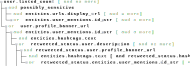
\includegraphics[width=\columnwidth]{SchemaSummarization/img/collapse-FPTree}
\caption{FP-Tree based schema summaries}
\label{fig:summary:fptree}
\end{figure}

\tinysection{FP-Tree Summaries}
An FP-Tree is a trie-like data structure that makes it easier to identify common patterns in a query.  
Every edge in the tree represents the inclusion of one feature, or in our case one attribute.
Hence, every node in the tree corresponds to a set of paths (obtained by traversal from the root), and every leaf corresponds to one source schema.
We observe that every node in an FP tree corresponds to a disjunction: For a node with 3 children, each subtree represents a different branch.  
Similarly, every edge corresponds to a conjunction with a singleton.
Although the resulting tree may duplicate some attributes, duplications are minimized~\cite{DBLP:conf/sigmod/HanPY00}.

\begin{example}
Figure~\ref{fig:summary:fptree} illustrates a schema summary based on  FP-Trees.  
Sequences of nodes with a single child are collapsed into single rows of the display (e.g., \inlinejson{user.listed_count} and 63 immediate descendents).
A toggle switch allows these entities to be displayed to the user, if desired.
Every level of the tree represents a set of alternatives. For example, \inlinejson{possibly_sensitive} never co-occurs with \inlinejson{user.profile_banner_url}.  
\end{example}

\tinysection{RCDC Summaries}
Our second visualization is based on correlations and anticorrelations.
To construct this visualization, we begin with the joint summary.
Recall that the joint summary has the form 
$$(P_1 \vee \emptyset)\;(P_2 \vee \emptyset)\;(P_3 \vee \emptyset)\;(P_4 \vee \emptyset)\ldots$$

We create a covariance matrix based on the probability of two attributes co-occurring in the schemas of one of our input \json records.  
Using this covariance matrix, hierarchical clustering~\cite{Johnson1967}, and a user-controlled threshold on the covariance, we cluster the attributes by parenthesizing.  For example, clustering might group $P_1$ with $P_2$ and likewise $P_3$ with $P_4$.
We can rewrite this formula as:
$$\approx (P_1P_2 \vee \emptyset)\;(P_3P_4 \vee \emptyset)\ldots$$
Observe that this formula omits schemas that the original formula captures (e.g., any schema including $P_1$ but not $P_2$).
However, because clustering ensures that attributes within a group co-occur frequently, there are comparatively few such schemas.

We next repeat the process with a new covariance matrix built using the frequency of co-occurrence of \emph{groups} (like $P_1P_2$).  
As before, we create clusters, but this time we cluster based on extremely negative co-variances.
Hence, members of the resulting clusters are unlikely to co-occur.
Continuing the example, let us assume that $P_1P_2$ and $P_3P_4$ are highly anti-correlated.  
Approximating and simplifying, we get an expression in RCDC form.
$$\approx (P_1P_2 \vee P_3P_4 \vee \emptyset)\ldots$$
As with the FP-Tree display, we use counts and an example attribute as a summary name for the group, and a toggle button to allow users to expand the group along either the OR or AND axes.

\begin{figure}
\centering
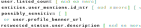
\includegraphics[width=0.8\columnwidth]{SchemaSummarization/img/collapse-RCDC}
\caption{RCDC based schema summaries}
\label{fig:summary:rcdc}
\end{figure}




